\documentclass{bmstu}

\bibliography{biblio}
\usepackage{enumitem}
\usepackage{amsmath,amssymb,amsthm}

\usepackage{algorithm}
\usepackage{algpseudocode}
\floatname{algorithm}{Алгоритм}
\captionsetup[ruled]{labelsep=period}
\makeatletter
\@addtoreset{algorithm}{chapter}% algorithm counter resets every chapter
\makeatother
\renewcommand{\thealgorithm}{\thechapter.\arabic{algorithm}}%

%Перевод команд псевдокода
\algrenewcommand\algorithmicwhile{\textbf{До тех пока}}
  \algrenewcommand\algorithmicdo{\textbf{выполнять}}
  \algrenewcommand\algorithmicrepeat{\textbf{Повторять}}
  \algrenewcommand\algorithmicuntil{\textbf{Пока выполняется}}
  \algrenewcommand\algorithmicend{\textbf{Конец}}
  \algrenewcommand\algorithmicif{\textbf{Если}}
  \algrenewcommand\algorithmicelse{\textbf{иначе}}
  \algrenewcommand\algorithmicthen{\textbf{тогда}}
  \algrenewcommand\algorithmicfor{\textbf{Цикл}}
  \algrenewcommand\algorithmicforall{\textbf{Выполнить для всех}}
  \algrenewcommand\algorithmicfunction{\textbf{Функция}}
  \algrenewcommand\algorithmicprocedure{\textbf{Процедура}}
  \algrenewcommand\algorithmicloop{\textbf{Зациклить}}
  \algrenewcommand\algorithmicrequire{\textbf{Условия:}}
  \algrenewcommand\algorithmicensure{\textbf{Обеспечивающие условия:}}
  \algrenewcommand\algorithmicreturn{\textbf{Вернуть}}
  \algrenewtext{EndWhile}{\textbf{Конец цикла}}
  \algrenewtext{EndLoop}{\textbf{Конец зацикливания}}
  \algrenewtext{EndFor}{\textbf{Конец цикла}}
  \algrenewtext{EndFunction}{\textbf{Конец функции}}
  \algrenewtext{EndProcedure}{\textbf{Конец процедуры}}
  \algrenewtext{EndIf}{\textbf{Конец условия}}
  \algrenewtext{EndFor}{\textbf{Конец цикла}}
  \algrenewtext{BeginAlgorithm}{\textbf{Начало алгоритма}}
  \algrenewtext{EndAlgorithm}{\textbf{Конец алгоритма}}
  \algrenewtext{BeginBlock}{\textbf{Начало блока. }}
  \algrenewtext{EndBlock}{\textbf{Конец блока}}
  \algrenewtext{ElseIf}{\textbf{иначе если }}

\begin{document}

\makereporttitle
    {Информатика, искусственный интеллект и системы управления} % Название факультета
    {Программное обеспечение ЭВМ и информационные технологии} % Название кафедры
    {лабораторной работе №~6} % Название работы (в дат. падеже)
    {Экспертные системы} % Название курса (необязательный аргумент)
    {Обратный дедуктивный вывод в обобщенных правилах продукции} % Тема работы
    {} % Номер варианта (необязательный аргумент)
    {Клименко~А.~К./ИУ7-31М} % Номер группы/ФИО студента (если авторов несколько, их необходимо разделить запятой)
    {Русакова~З.~Н.} % ФИО преподавателя

\chapter*{Введение}

Цель лабораторной работы --- приобретение практических навыков реализации алгоритма обратного дедуктивного вывода на обобщенных правилах продукции.

Задачи работы:
\begin{enumerate}
    \item Формализовать алгоритм обратного дедуктивного вывода.
    \item Разработать программу, реализующую алгоритм обратного дедуктивного вывода.
    \item Протестировать программу на различных логических программах.
\end{enumerate}


\chapter{Теоретический раздел}

\section{Обобщенное правило продукции}

Пусть $x$ --- задан на конкретном множестве, а $c$ --- объект этого множества, тогда
$$\frac{A(c), A(x) \rightarrow B(x)}{B(c)}.$$

В общем случае, если в посылке конъюнкция и заданы подстановки для каждого $P_i$, то мы можем получить композицию подстановок.

Отсутствие направления вывода в методе резолюции называется \textbf{потерей импликативности}.
Импликативный вывод используется для простых случаев.

\section{Система дедукции на основе обобщенных правил продукции}

Определенное выражение является либо атомарным (атомом), либо представляет собой импликацию антицидентом (предпосылкой) которой является конъюнкция положительных атомов, а консеквент --- единственный положительный атом.

В определенных выражениях в базе знаний не используются функциональные символы, но определенные выражения содержат направление вывода, что намного повышает эффективность систем вывода и упрощает его. Метод резолюции позволяет обработать более сложные представления знаний, что определенные выражения не всегда позволяют, но процедура резолюции влечет потерю импликативности, то есть нет направления вывода.

Пример:
\begin{eqnarray*}
  (\neg A \& \neg B) &\rightarrow& C, \\
  (\neg B \& \neg C) &\rightarrow& A
\end{eqnarray*}
дают одинаковые дизъюнкты, но видим, что в исходных формулах разное направление вывода.

\section{Алгоритм обратного дедуктивного вывода}

Обратная дедукция для базы знаний из определенных выражений производится методом поиска в глубину. Структуры данных: переменные, константы, атом. База правил представлена списком правил. Правило содержит список входных атомов, которые соответствуют входным вершинам, один выходной атом (выходная вершина), номер правила, флаг доказано/недоказано и метку (выбрано или нет). В атоме тоже вводится флаг (помимо списка переменных) доказан атом или не доказан. Факты --- это атомы, в которых стоят константы. Они соответствуют закрытым вершинам в графах И-ИЛИ (мы их задаем) и еще есть целевой атом (целевая вершина). Возможно что целевой атом имеет константы, а может не имеет.

Целевой атом записываем в голову стека. Факты записываем в список закрытых вершин. В процессе поиска формируем стек открытых вершин (атомов); список подстановок для текущего шага; список закрытых атомов / закрытых вершин, которые добавляются к исходному списку фактов; список закрытых правил, которые содержат дерево решения.

Метод поиска остается без изменений. Пока оба флага выставлены в единицу, вызываем метод потомков на каждом шаге поиска. Изменяется метод потомков и метод разметки. В этих методах необходимо проводить унификацию и формировать подстановки. В методе потомков выполняется унификация атома подцели (из стека) и выходной атом рассматриваемого правила. Унифицируются подцель и выходной атом правила. Если унификация успешна, то формируем подстановки. Причем, константа может стоять как в подцели так и в выходном атоме правила. Если выходной атом получает константу, то её необходимо распространить на все атомы рассматриваемого правила, в которое входит переменная, получившая константу. Если константу получают переменные подцели, то она ставится в подцель. При этом можно рассмотреть 2 пути: если подцель получила константу, то распространить эту константу на оставшиеся в стеке атомы последнего правила. Альтернатива --- можно не распространять константу из подцели, а оставить их с переменными, --- они получат значения потом при их доказательстве.

Итог: выбираем подцель, находим первое правило, у которого подцель унифицируется с выходной вершиной. Нам нужно проверить, сколько атомов у этого правила уже закрыто (входные вершины доказаны). Для этого мы каждый атом входной проверяем, не находится ли он в базе. Если он есть, то его переменные получают значения. Эти значения распространяем в другие атомы. В стек записываем только те атомы, которые не закрываются фактами. Если мы записали подцели, то номер правила помещаем в список открытых правил.

Подстановка необходима на одном шаге раскрытия подцели и формирования новых подцелей. Потом она уже не нужна, но можно использовать.

Следующий шаг --- если у найденного правила все атомы доказаны. Это правило добавляем в список закрытых и начинаем разметку. В разметке мы должны выходную вершину правила добавить к фактам. В результате подстановки, мы должны полученные значения переменных предыдущих правил распространить на эти же переменные в оставшихся недоказанных атомах (если они есть). Идет обратное распространение переменных (снизу вверх в подцели). Соответственно, из головы стека подцель удаляем. Если недоказанные атомы для последнего правила были, то вызываем потомков. Если недоказанных атомов больше нет, то продолжаем цикл разметки.

Рассмотрим построение для наших правил.

Факты:
\begin{enumerate}
  \item $O(N,M1)$
  \item $M(M1)$
  \item $A(W)$
  \item $E(N,A1)$
\end{enumerate}

Правила:
\begin{enumerate}
  \item $A(x) \& W(y) \& S(x, y, z) \& H(z) \rightarrow C(x)$
  \item $M(x_2) \& O(N, x_2) \rightarrow S(W, x_2, N)$
  \item $M(x_1) \rightarrow W(x_1)$
  \item $E(x_3, A1) \rightarrow H(x_3)$
\end{enumerate}

Цель: $C(x_0)$

Шаги:
\begin{enumerate}
  \item стек: $[ C(x_0) ]$

  $C(x_0)$ унифицируется с выходным атомом правила 1. Подстановка: $\{x_0/x\}$
  Мы должны проверить, какие атомы этого правила закрыты. Берем $A(x)$ ищем в базе фактов, находим $A(W)$ --- $x$ заменяется на константу $W$. Распространяем переменную на остальные факты. $A(W)$ в стек не пишем, рассматриваем следующую подцель. $W(y)$ в базе фактов нет, поэтому кладем в стек:
	
  стек: $[ W(y), S(W,y,z), H(z), C(W) ]$

  \item второй шаг метода потомков --- $W(y)$ унифицируется с выходом правила 3. Подстановка: $\{y/x_1\}$. Нам нужно проверить у этого правила, какие вершины не доказаны и что писать в стек, в нашем случае при доказательстве он сопоставляется с фактом $M(M1)$, когда мы будем доказывать  входную вершину получим подстановку $\{M1/y\}$. Правило 3 закрываем. Добавляем факт $W(M1)$ в базу фактов. Распространяем подстановку $\{M1/y\}$ на оставшиеся атомы.

	стек: $[ S(W, M1, z), H(z), C(W) ]$, а в базе фактов новый факт: $W(M1)$. \\
	Из разметки вышли --- $W(y)$ убираем, а недоказанные подцели есть. Теперь будем доказывать $S(W, M1, z)$.

  \item В результате унификации $S(W,M1,z)$ с выходом правила $S(W, x_2, N)$ надо распространять в оба направления --- $x_2$ вниз (в подцели для $S$), $z$ вправо (в $H(z)$). Подцели $S$ будут доказаны из фактов, из этого следует, что вершина $S(W, M1, N)$ --- новый факт, который мы добавим в базу фактов и уберем из стека.

  \item Подцель $H(N)$. Правило 4. Входной модуль $E(x_3, A1)$. В результате распространения получаем $E(N, A1)$. Такой факт у нас есть. $H(N)$ в новые факты, убираем из стека.
  
  \item Вызываем разметку для $C(W)$ --- удаляем из стека. Стек пуст --- исходное утверждение доказано.
\end{enumerate}

\chapter{Практический раздел}

База правил хранит список правил. Факты представлены структурой правила с пустым списком входных атомов.

\section{Формализация алгоритма обратного дедуктивного вывода}

Алгоритм обратного дедуктивного вывода \textbf{Backward-ASK} работает на основе генераторов для обеспечения поиска всех возможных решений для цели с возможностью приостановки поиска. Главная идея алгоритма --- обратный поиск в глубину в графе И-ИЛИ с использованием двух процедур --- \textbf{Backward-OR} и \textbf{Backward-AND}.

\begin{algorithm}[h!]
  \caption{\textbf{Backward-ASK}. Алгоритм обратного дедуктивного вывода}
  \label{alg:backward-ask}
  \hspace*{\algorithmicindent} \textbf{Вход:} \textit{KB} --- база правил, \textit{цель} --- атом. \\
  \hspace*{\algorithmicindent} \textbf{Выход:} генератор подстановок
  \begin{algorithmic}[1]
  \\
  \Return Backward-OR (\textit{KB}, \textit{цель}, \{\})
  \end{algorithmic}
\end{algorithm}

Процедура \textbf{Backward-OR} производит перебор правил, которые \textit{разрешают} текущую подцель (то есть выходная вершина которых унифицируется с текущей подцелью), и после переименования переменных в найденном правиле вызывает процедуру \textbf{Backward-AND} для доказательства входных атомов текущего правила с применением подстановки, полученной в процессе унификации заключения текущего правила и текущей подцели. Если текущее правило оказалось фактом, его посылка будет пуста. Эту ситуацию обработает процедура \textbf{Backward-AND}.

\begin{algorithm}[h!]
  \caption{\textbf{Backward-OR}. Алгоритм перебора правил ИЛИ}
  \label{alg:backward-or}
  \hspace*{\algorithmicindent} \textbf{Вход:} \textit{KB} --- база правил, \textit{подцель} --- атом, $\theta$ --- базовая подстановка. \\
  \hspace*{\algorithmicindent} \textbf{Выход:} генератор подстановок
  \begin{algorithmic}[1]
  \For{по всем \textit{правилам} $\gets KB$ разрешающим \textit{подцель}}
    \State (\textit{посылка} $\Rightarrow$ \textit{заключение}) $\gets$ \textbf{STD-VAR}(\textit{правило})
    \For{$\theta' \in$ \textbf{Backward-AND}(\textit{KB}, \textit{посылка}, \textbf{UNIFY}(\textit{заключение}, \textit{подцель}, $\theta$))}
      \State \textbf{Выбросить} подстановку $\theta'$
    \EndFor
  \EndFor
  \end{algorithmic}
\end{algorithm}

Функция \textbf{STD-VAR} выполняет переименование переменных входного правила и возвращает новое правило.

Функция \textbf{UNIFY} производит унификацию двух атомов с заданной подстановкой и возвращает новую подстановку. В случае невозможности унификации, функция возвращает ошибку.

Процедура \textbf{Backward-AND} выполняет доказательство входного списка подцелей. Для этого выполняется перебор всех возможных подстановок для первой подцели с использованием процедуры \textbf{Backward-OR}. Затем выполняется рекурсивный вызов для доказательства остальных подцелей с полученной подстановкой.

\begin{algorithm}[h!]
  \caption{\textbf{Backward-AND}. Алгоритм перебора правил И}
  \label{alg:backward-and}
  \hspace*{\algorithmicindent} \textbf{Вход:} \textit{KB} --- база правил, \textit{подцели} --- список атомов, $\theta$ --- базовая подстановка. \\
  \hspace*{\algorithmicindent} \textbf{Выход:} генератор подстановок
  \begin{algorithmic}[1]
    \If{$\theta$ --- ошибка} \Return
    \ElsIf {список \textit{подцелей} пуст}
      \State \textbf{Выбросить} подстановку $\theta$
    \Else
      \State \textit{голова}, \textit{хвост} $\gets$ список \textit{подцелей}
      \For{$\theta' \in$ \textbf{Backward-OR}(\textit{KB}, \textbf{SUBST}(\textit{голова}, $\theta$), $\theta$)}
        \For{$\theta'' \in$ \textbf{Backward-AND}(\textit{KB}, \textit{хвост}, $\theta'$)}
          \State \textbf{Выбросить} подстановку $\theta''$
        \EndFor
      \EndFor
    \EndIf
  \end{algorithmic}
\end{algorithm}

Функция \textbf{SUBST} применяет подстановку к входному атому и возвращает новый атом.

Рассмотрим пример работы описанного алгоритма обратного дедуктивного вывода. Пусть база знаний содержит следующие правила (факты являются частными случаями правил):
\begin{eqnarray}
  B(y, W) ~\&~ C(x, K, y) &\rightarrow& A(x, y), \\
  D(y) ~\&~ E(x, K) &\rightarrow& B(x, y), \\
  B(z, x) ~\&~ E(y, z) &\rightarrow& C(x, y, z), \\
  && D(W), \\
  && E(K, K).                     
\end{eqnarray}

Цель: $A(r, s)$.

\begin{figure}[ht!]
  \centering
  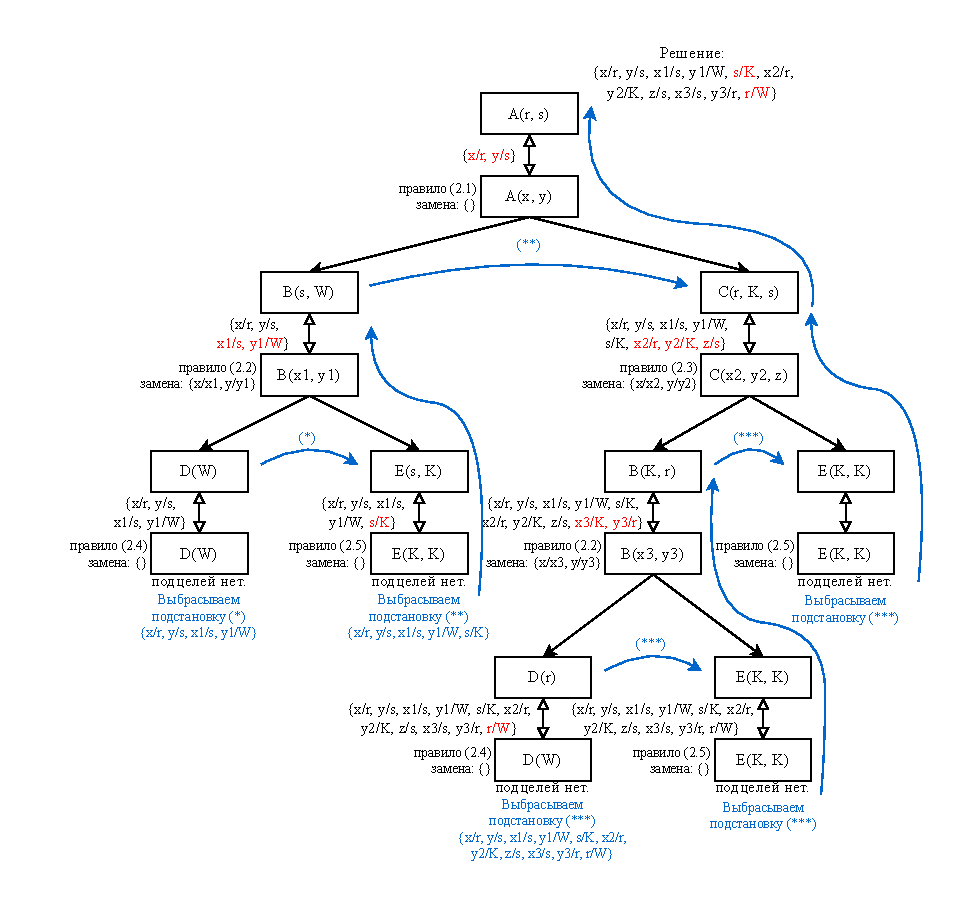
\includegraphics[width=\linewidth]{backward-ask-1.pdf}
  \caption{Пример простой схемы вывода}
  \label{fig:ask1}
\end{figure}

Cхема вывода показана на рисунке \ref{fig:ask1}. Синим цветом указано направление передачи выбрасываемых подстановок из генераторов.

\section{Поиск всех допустимых подстановок}

Рассмотрим другой пример, иллюстрирующий возврат. Пусть база знаний состоит из следующих правил:
\begin{eqnarray}
Mark(st, sub, 5) ~\&~ Mark(st, sub, 4) &\rightarrow& GoodAt(st, sub) \\
Mark(Alice, Maths, 4) \\
Mark(Alice, Maths, 5) \\
Mark(Bob, Maths, 3) \\
Mark(Bob, Maths, 4) \\
Mark(Carl, Phys, 5) \\
Mark(Carl, Phys, 4) \\
Mark(Alice, Phys, 4) \\
Mark(Bob, Phys, 4) \\
Mark(Bob, Phys, 3)
\end{eqnarray}

Цель --- найти все такие пары <<студент--предмет>>, что студент $st$ имеет оценки 4 и 5 по предмету $sub$. То есть найти все возможные подстановки для предиката $GoodAt(st, sub)$. Схема перебора допустимых подстановок представлена на рисунке \ref{fig:ask2}.

\begin{figure}[ht!]
  \centering
  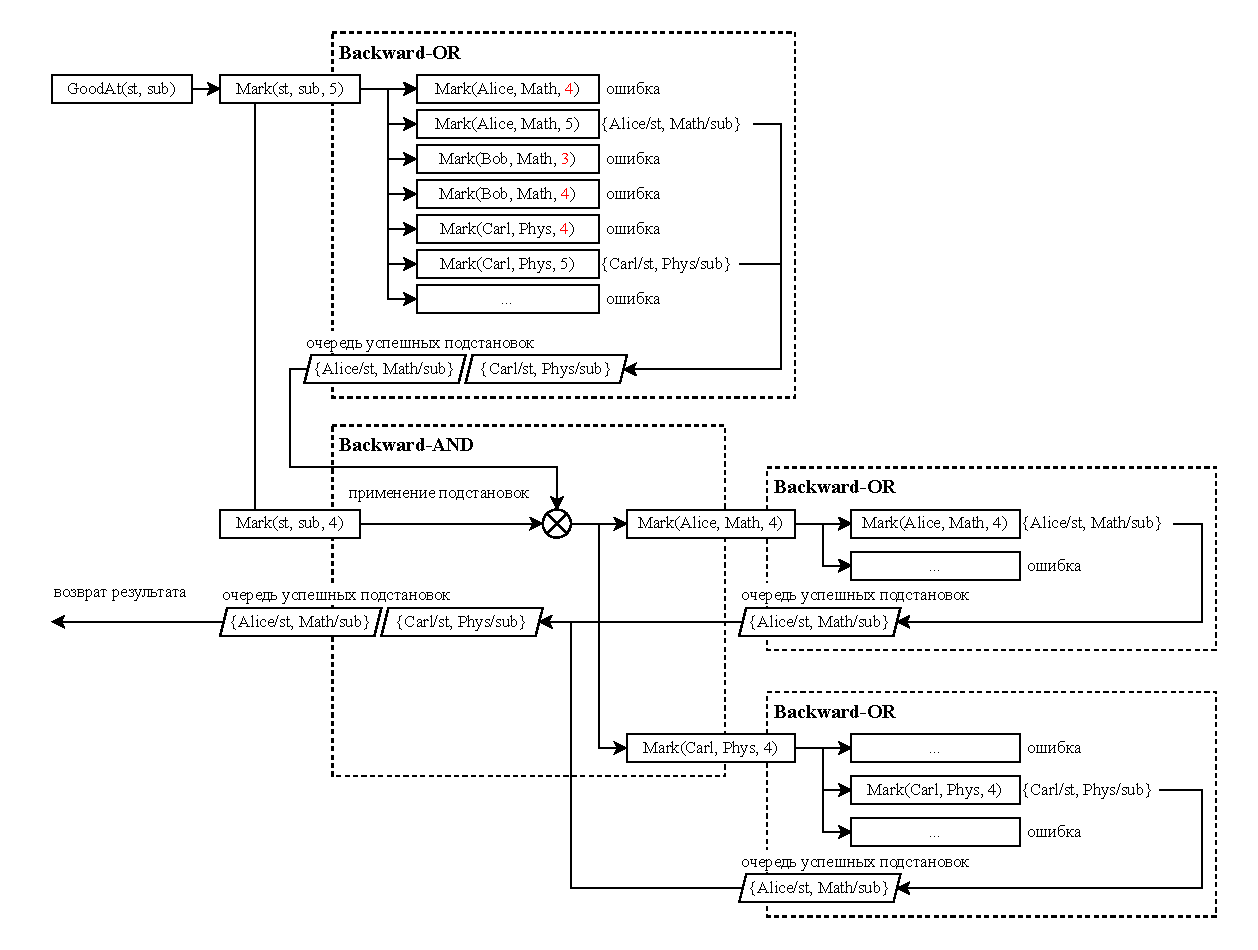
\includegraphics[width=\linewidth]{backward-ask-2.pdf}
  \caption{Схема перебора всех допустимых подстановок}
  \label{fig:ask2}
\end{figure}

\section{Отсечение дерева решений}

Отсечение дерева решений реализуется введением дополнительного флага, передаваемого через очередь подстановок. Так как оператор отсечения может встретиться только в антициденте некоторого правила, то флаг отсечения должен генерироваться в процедуре \textbf{Backward-AND}. Как только первый атом из списка входных подцелей является оператором отсечения, процедура \textbf{Backward-AND} выбрасывает вместо подстановки специальный флаг, после чего продолжает свое выполнение пропустив первый элемент в списке подцелей (оператор отсечения).

Обработать флаг отсечения вместо подстановки может только процедура \textbf{Backward-OR}. При получении данного флага в процедуре запрещается дальнейший перебор правил базы знаний. 

\section{Механизм специальных процедур}

Иногда значение истинности некоторого предиката не может быть выражено с использованием только лишь определенных выражений, или их количество может быть бесконечно большим. В таком случае можно ввсети таблицу, определяющую соответствие между именем предиката и некоторым объектом, которому будет делегирована задача по доказательству этого предиката. Описанная проверка производится в начале процедуры \textbf{Backward-OR}.

В данной работе реализованы следующие специальные процедуры:
\begin{enumerate}
  \item \texttt{write(...)} --- выводит значения аргументов в консоль, всегда истиннен.
  \item \texttt{add(x, y, z)} $\Leftrightarrow x + y = z$. Может вычислить одну переменную.
  \item \texttt{mul(x, y, z)} $\Leftrightarrow x * y = z$. Может вычислить одну переменную.
  \item \texttt{leq(x, y)} $\Leftrightarrow$ $x$ и $y$ связаны с целыми числами и $x \le y$.
  \item \texttt{in\_range(var, start, end)} --- если все агрументы связаны с целыми числами, то истинность определяется условием $start \le var < end$; если $var$ --- свободная переменная, а $start$ и $end$ связаны с целыми числами, то генерирует последовательность подстановок $\{i/var\}_{i=start}^{end-1}$.
\end{enumerate}

Используя последний предикат \texttt{in\_range} можно организовать последовательный перебор чисел. Например, следующая программа выведет в столбик все уникальные пары чисел от 1 до 10 не включительно:
\begin{verbatim}
  nums(x,y) :- in_range(v,x,y), in_range(u,v,y), write(v,u), fail
  ?- nums(1, 10)
\end{verbatim}

\section{Сборка и запуск ПО}

Для сборки программы используется \texttt{CMake}. Стандартная последовательность команд для сборки и запуска программы:

\begin{verbatim}
mkdir build && cd build && cmake ..
make app && ./app # сборка и запуск программы
make unittests && ./unittests # опциональный запуск юнит-тестов
\end{verbatim}

Альтернативно, можно собрать и запустить программу с помощью \texttt{makefile} скрипта в корневой папке используя цель <<\texttt{app}>>.

При запуске основной программы (app) первым аргументом можно указать путь к файлу, содержащему правила базы знаний. По-умолчанию программа работает с пустой базой знаний.

Основная программа работает в интерактивном режиме. Для добавления правила в базу знаний необходимо написать символ <<\texttt{+}>> и текст самого правила. Для запуска алгоритма дедуктивного вывода достаточно написать атом. При этом запустится алгоритм прямого дедуктивного вывода. Для запуска алгоритма обратного дедуктивного вывода необходимо ввести символ <<\texttt{!}>> перед атомом.

Пример работы программы:
\begin{verbatim}
?- +P(x, y) :- Q(x), R(y)       # добавление правила
>> P(x1, y1) :- Q(x1), R(y1)
?- +R(A)                        # добавление фактов
>> R(A)
?- +Q(B)
>> Q(B)
?- P(a, b)                      # прямой вывод
{a=B, b=A}                      # результат - подстановка
next?- y                        # запрос продолжения поиска
end                             # больше решений нет
?- !P(r, s)                     # обратный вывод
{r=B, s=A}
next?-
\end{verbatim}

\section{Тестирование ПО}

Для тестирования разработанного ПО были разработаны логические тесты, представленные в таблицах \ref{tbl:tests-1}--\ref{tbl:tests-2}.

\begin{table}[ht]
  \caption{Тестовые программы (часть 1)}
  \label{tbl:tests-1}
  \centering
  \begin{tabular}{|l|l|}
    \hline
    \textbf{№} & \textbf{Правила теста} \\
    \hline
    \hline
    1 & Поиск максимума из трех чисел \\
    \hline
    & \texttt{max(a, b, c, a) :- less(b, a), less(c, a)} \\
    & \texttt{max(a, b, c, b) :- less(a, b), less(c, b)} \\
    & \texttt{max(a, b, c, c) :- less(a, c), less(b, c)} \\
    & \texttt{less(1, 2)} \\
    & \texttt{less(2, 3)} \\
    & \texttt{less(1, 3)} \\
    \hline
    & Запрос: \texttt{max(1, 3, 2, x)} \\
    & Результат: \texttt{\{x=3\}} \\
    \hline
    \hline
    2 & Определение длины списка \\
    \hline
    & \texttt{len(Nil, 0) :- !} \\
    & \texttt{len(cons(\_, x), succ(n)) :- len(x, n)} \\
    \hline
    & Запрос: \texttt{len(cons(A, cons(B, cons(C, Nil))), x)} \\
    & Результат: \texttt{\{x=succ(succ(succ(0)))\}} \\
    \hline
    \hline
    3 & Генерация списка заданной длины \\
    \hline
    & \texttt{len(Nil, 0) :- !} \\
    & \texttt{len(cons(\_, x), succ(n)) :- len(x, n)} \\
    \hline
    & Запрос: \texttt{len(x, succ(succ(succ(0))))} \\
    & Результат: \texttt{\{x=cons(\_, cons(\_, cons(\_, Nil)))\}} \\
    \hline
  \end{tabular}
\end{table}

\begin{table}[ht]
  \caption{Тестовые программы (часть 2)}
  \label{tbl:tests-2}
  \centering
  \begin{tabular}{|l|l|}
    \hline
    \textbf{№} & \textbf{Правила теста} \\
    \hline
    \hline
    4 & Реверс списка \\
    \hline
    & \texttt{reverse(Nil, Nil) :- !} \\
    & \texttt{reverse(x, y) :- reverse\_helper(x, y, Nil)} \\
    & \texttt{reverse\_helper(Nil, x, x)} \\
    & \texttt{reverse\_helper(cons(h, r), x, y) :-} \\
    & \texttt{    reverse\_helper(r, x, cons(h, y))} \\
    \hline
    & Запрос: \texttt{reverse(cons(A, cons(B, cons(C, Nil))), x)} \\
    & Результат: \texttt{\{x=cons(C, cons(B, cons(A, Nil)))\}} \\
    \hline
    \hline
    5 & Лабиринт \\
    \hline
    & \texttt{\# +-\--\--+-\--\--+-\--\--+} \\
    & \texttt{\# | 1 |X2X|X3X|} \\
    & \texttt{\# +-\--\--+-\--\--+-\--\--+} \\
    & \texttt{\# | 4 | 5 | 6 |} \\
    & \texttt{\# +-\--\--+-\--\--+-\--\--+} \\
    & \texttt{\# | 7 |X8X| 9 |} \\
    & \texttt{\# +-\--\--+-\--\--+-\--\--+} \\
    & \texttt{step(1, 4)} \\
    & \texttt{step(4, 5)} \\
    & \texttt{step(4, 7)} \\
    & \texttt{step(5, 6)} \\
    & \texttt{step(6, 9)} \\
    & \texttt{way(x, y) :- step(x, y)} \\
    & \texttt{way(x, y) :- step(x, z), way(z, y)} \\
    \hline
    & Запрос: \texttt{way(1, w)} \\
    & Результат: \texttt{\{w=4\}, \{w=5\}, \{w=7\}, \{w=6\}, \{w=9\}} \\
    \hline
    \hline
    6 & Различность \\
    \hline
    & \texttt{neq(x, x) :- !, fail} \\
    & \texttt{neq(\_, \_)} \\
    \hline
    & Запрос: \texttt{neq(A, A)} \\
    & Результат: \texttt{no} \\
    \hline
    & Запрос: \texttt{neq(A, B)} \\
    & Результат: \texttt{\{\}} \\
    \hline
  \end{tabular}
\end{table}

\clearpage

В таблице \ref{tbl:tests-3} представлены тесты, включающие в себя работу со специальными процедурами, описанными в разделе 2.4.

\begin{table}[ht]
  \caption{Тестовые программы (часть 3)}
  \label{tbl:tests-3}
  \centering
  \begin{tabular}{|l|l|}
    \hline
    \textbf{№} & \textbf{Правила теста} \\
    \hline
    \hline
    7 & Отображение пути вывода \\
    \hline
    & \texttt{\# leq(x, y)} $\Leftrightarrow x \le y$ --- спец. процедура \\
    & \texttt{\# write(...)} --- спец. процедура \\
    & \texttt{min(a, b, a) :- write(First, Route), leq(a, b), !} \\
    & \texttt{min(\_, b, b) :- write(Second, Route)} \\
    \hline
    & Запрос: \texttt{min(14, 50, x)} \\
    & Результат: \texttt{\{x=14\}} \\
    & Побочный эффект (вывод на экран): \\
    & ~~~\texttt{First Route} \\
    \hline
    & Запрос: \texttt{min(3, 2, x)} \\
    & Результат: \texttt{\{x=2\}} \\
    & Побочный эффект (вывод на экран): \\
    & ~~~\texttt{First Route} \\
    & ~~~\texttt{Second Route} \\
    \hline
    \hline
    8 & Определение простоты числа \\
    \hline
    & \texttt{\# mul(x, y, z)} $\Leftrightarrow x * y = z$ --- спец. процедура \\
    & \texttt{\# in\_range(a, b, c)} --- спец. процедура \\
    & \texttt{divisible(x, y) :- mul(z, y, x), mul(z, y, x), !} \\
    & \texttt{composite(x) :- in\_range(v, 2, x), divisible(x, v), !} \\
    & \texttt{prime(1) :- !, fail} \\
    & \texttt{prime(x) :- composite(x), !, fail} \\
    & \texttt{prime(\_)} \\
    \hline
    & Запрос: \texttt{prime(5)} \\
    & Результат: \texttt{\{\}} \\
    \hline
    & Запрос: \texttt{prime(12)} \\
    & Результат: \texttt{no} \\
    \hline
  \end{tabular}
\end{table}

\chapter*{Выводы}

В ходе лабораторной работы была разработана программа реализующая алгоритм обратного дедуктивного вывода с возможностью полного перебора допустимых решений. Добавлена поддержка оператора отсечения, а также реализован механизм вызова специальных процедур.

В качестве направлений для дальнейшего развития алгоритма и программы можно выделить следующие:
\begin{itemize}[label=---]
  \item aнализ зависимостей по переменным и параллелизация доказательства независимых предикатов;
  \item реализация вычислимых функциональных символов;
  \item добавление специальных процедур для работы с вводом-выводом.
\end{itemize}


\end{document}